%!TEX root = ../dokumentation.tex
\lstset{
	frame=single,
	keywordstyle=\color{blue},
	commentstyle=\color{green},
	numbers=left,
}

\part{Implementierung}

\chapter{Frontend}
Nachdem in den bisherigen Kapiteln eher die technischen und theoretischen Grundlagen diskutiert wurden, wird nun die eigentliche Implementierung des \textbf{Sudoku Solver} erläutert.

Zunächst wird das Frontend mit allen Funktionalitäten des User Interfaces und der daraus resultierenden User Experience, sowie die Umsetzung der einzelnen Hilfestellungen beschrieben.

Das Frontend ist letztlich alles was der User auf der Website sehen kann. Alles was der Nutzer nicht sehen kann gehört zum Backend. Trotzdem ist das Frontend sehr entscheidend, denn es sollte möglichst Benutzerfreundlich sein. Dazu gehört eine intuitive Nutzung der Oberfläche und im Falle des \textbf{Sudoku Solver} das übersichtliche Anzeigen der Lösungsstrategie und die Erklärung dazu, sowie die sprechende Markierung auf dem Sudokuboard.

\section{\acl{UI}}
Das \ac{UI} ist die Nutzerschnittstelle zum Backend. An dieser Stelle beeinflusst der Nutzer durch seine Handlung die Reaktion im Backend und wie das Frontend letztlich wieder auf diese Handlung reagiert. An dieser Stelle der Ausarbeitung werden die Designentscheidungen für das \ac{UI} vorgestellt. Daher wird im Folgenden die \ac{HTML} Struktur und das darauf basierende responsiv Design beschrieben.

Ein wichtiger Teil des \ac{UI} ist es, dem Nutzer alle Funktionalitäten übersichtlich und klar zur Verfügung zu stellen. Wenn das \ac{UI} schon unübersichtlich und schlecht zu verstehen ist, dann wird auch die \acs{UX} keine gute sein, egal wie gut die Software im Backend letztlich ist. Eine weitere Anforderung an das Frontend ist das responsiv Design. Die Website soll sich möglichst allen Formaten anpassen und auf verschiedenen Endgeräten ihren passend skaliert werden.

\subsection{\ac{HTML} Struktur}
Die \ac{HTML} Datei ist unterteilt in \textit{<head>} und \textit{<body>}. 

Im Head werden Informationen über die Seite, wie beispielsweise der Titel oder die Stylesheets definiert. Ebenso werden die benutzten Skripts aus den externen Dateien in das Dokument eingebunden. 

Im Body sind die darzustellenden Inhalte eines \ac{HTML} Dokuments enthalten und weil das Produkt hauptsächlich auf einem Computer genutzt wird, ist die \ac{HTML} Struktur im Body darauf angepasst.

In der Abbildung \ref{fig:AbbildungFrontend} ist das Frontend zu sehen. Das Sudokuboard, das NumPad und die Erläuterung der Strategie liegen jeweils nebeneinander. Das Sudokuboard wird rechts und in einer zur Browsergröße passenden Höhe abgebildet, damit alle Zahlen gut zu sehen sind. Rechts daneben wird das NumPad platziert. Dadurch ist, durch den Platzhalter für die Erläuterung der Strategie, keine Lücke zwischen den Objekten, die für die Nutzerinteraktion relevant sind. Um das NumPad nicht zu verschieben wenn ein Titel einer Strategie angezeigt wird, hat das Feld für Titel und Erklärung einen festen Platzhalter rechts neben dem NumPad.

Die Lösung ist dabei so aufgebaut, dass das Sudokuboard in einem Div liegt und das NumPad mit dem Textfeld in einem weiteren. Dieses Div von NumPad und Textfeld ist nochmal in zwei Divs unterteilt. In der folgenden Abbildung \ref{fig:AbbildungFrontend} ist die Unterteilung der Elemente nochmals visualisiert.

\begin{figure}[htbp]
	\centering
	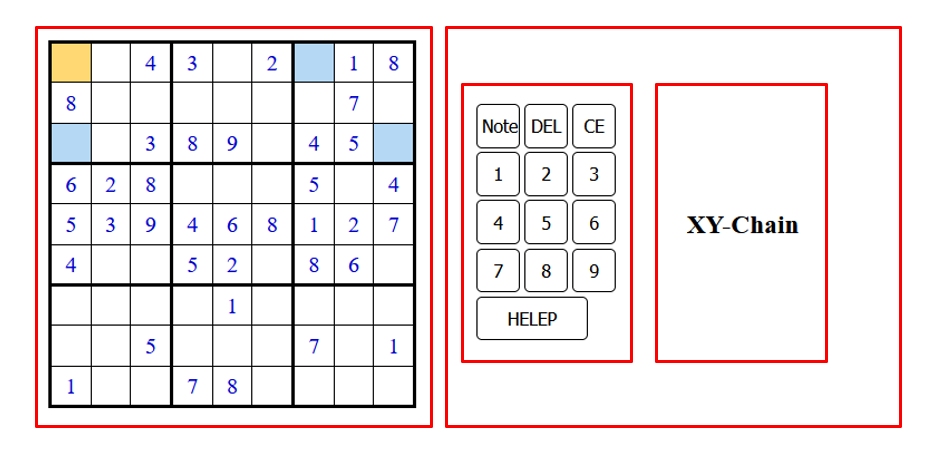
\includegraphics[width=0.8\textwidth]{images/AbbildungFrontendRot.png}
	\caption{\ac{HTML} Struktur des Frontend}
	\label{fig:AbbildungFrontend}
\end{figure}

\subsection{Responsiv Design}

Die in der \ac{HTML} Struktur beschriebenen Designentscheidungen wurden hauptsächlich von dem Responsiv Design beeinflusst. 

Den Elementen wird die Layoutmethode der Flexbox gegeben. Damit werden Elemente automatisch gestreckt, wenn es mehr Platz zum Füllen gibt und sie werden gestaucht, wenn es weniger Platz gibt. Mit den Flexboxen ist es daher relativ einfach möglich ein responsiv Design zu schaffen. 

Wenn das Fenster kleiner wird, dann skaliert sowohl das Board als auch das NumPad und das Textfeld mit. Falls das Fenster zu schmal wird, sodass Board und Kombination aus NumPad und Textfeld nebeneinander kein Platz haben, dann wird das Element von NumPad und Textfeld unter dem Board angezeigt.

Insgesamt wird das Board so skaliert, dass der Nutzer in der horizontalen nicht scrollen muss, um das gesamte Board zu sehen. Das ist aber nur bis zu einer gewissen Breite sinnvoll, da sonst das Board zu klein wird. Diese Breite wurde basierend auf dem Frontend eines mobilen Endgeräts bestimmt.

In der Flexbox von NumPad und Textfeld sind beide Divs jeweils nochmal eigene Flexboxen. Im anderen Fall ergab sich das Problem, dass die Position des NumPad abhängig von der Stufe der Hilfestellung flexibel ist. Das ergab keine gute \ac{UX}. Durch diese beiden Flexboxen ist auch das Anzeigen bei schmaleren Fenstern einfacher geworden. In diesem Fall wird das NumPad und die Erläuterung nebeneinander unter dem Board angezeigt wie in Abbildung \ref{fig:Responsiv} dargestellt. Die Flexbox von von NumPad und Textfeld ist dabei genauso breit wie das Board selbst.

\begin{figure}[htbp]
	\centering
	\includegraphics[width=0.5\textwidth]{images/Bilduntereinander.png}
	\caption{Responsiv Frontend}
	\label{fig:Responsiv}
\end{figure}

Ein weiterer Punkt der beim responsiv Design beachtet werden muss, ist die Schriftgröße. Eine Anpassung wird deshalb bei den Zahlen und Kandidaten auf dem Board und auch bei der Größe der Tasten des NumPad und die Schrift darauf vorgenommen. Das Gleiche gilt für das Textfeld mit Lösungsstrategie und Erläuterung. Die Skalierung der Schriftgröße wird in der \ac{CSS} Datei über viewports designt. Damit die Schrift am Ende nicht zu klein ist, wird eine \textit{min-font-size} definiert. 


\section{\acl{UX}}
Der folgende Abschnitt ist eine Ausführung über verschiedene Funktionalitäten, die für eine guten \acl{UX} implementiert sind. Dabei wird unterschieden zwischen den Funktionalitäten vom NumPad und anderen Eingaben und den Funktionalitäten des Sudokuboards.

Neben einer übersichtlichen und verständlich aufgebauten \ac{UI} muss noch eine gute \ac{UX} für ein gutes Frontend garantiert werden. Dazu gehören die Funktionalitäten der Knöpfe und eine angenehme Auswahl an Farben zur Markierung, um dem User die Nutzung der Website möglichst angenehm zu gestalten. Zum Beispiel gibt es für das Eintragen der Zahlen auf dem Sudoku verschiedene Varianten um eine gute \ac{UX} zu erreichen. 

\subsection{Funktionalitäten NumPad und andere Eingaben}
Es gibt auf de \ac{UI} ein NumPad mit verschiedenen Tasten. Wenn das Sudoku noch nicht gestartet wurde, unterscheidet sich die Anordnung der Knöpfe. Am Anfang sind in der obersten Reihe auf dem NumPad die Tasten Start, \ac{CE} und Del zu sehen. 

Beim Drücken des Startknopf wird zuerst die eindeutige Lösbarkeit des Rätsels geprüft. Wenn ein Sudoku nicht eindeutig lösbar ist, dann wird das dem Nutzer angezeigt. Falls es aber eindeutig Lösbar ist, verschwindet der Start Button und wird durch einen Note Knopf ersetzt. Zudem erscheint unter dem NumPad ein Help Knopf. Die Zahlen die zum Zeitpunkt des Drücken eingegeben wurden, bekommen eine andere Farbe und sind fest auf dem Board eingetragen. 

Mit der Taste \ac{CE} wird das komplette Sudokuboard zurückgesetzt. Mit eingeschlossen ist damit der Reset vom Starten des Sudokus und der Help Knopf verschwindet wieder. Wenn das Sudoku noch nicht gestartet wurde, werden nur die Zahlen auf dem Board entfernt. Mit der Del Taste werden in den ausgewählten Zellen der Eintrag gelöscht. Über die Note Taste wird der aktuelle Stand der Kandidaten angezeigt. Durch das mehrmalige Drücken des Help Knopf werden die abgestuften Hilfestellung angezeigt.

Für alle Funktionalitäten des NumPad wurden auch Tasten auf der Tastatur definiert. In der Tabelle \ref{tab:tastatur} werden die Funktionalitäten zu den Keys aufgezählt. Die Codierung wird im Hintergrund verwendet, um herauszufinden welche Taste gedrückt wurde.

% Please add the following required packages to your document preamble:
% \usepackage{graphicx}
\begin{table}[H]
	\centering
	\begin{tabular}{lll}
		\hline
		Key         & Code    & Funktionalität                     \\ \hline
		1..9        & 97..105 & Zahlen einfügen                    \\
		1..9        & 49..57  & Zahlen einfügen                    \\
		left arrow  & 37      & Pointer nach links bewegen         \\
		up arrow    & 38      & Pointer nach oben bewegen          \\
		right arrow & 39      & Pointer nach rechts bewegen        \\
		down arrow  & 40      & Pointer nach unten bewegen         \\
		shift       & 16      & Notes anzeigen                     \\
		space       & 32      & Zelle klicken                      \\
		tab         & 9       & Pointer zur nächsten Zelle bewegen \\
		delete      & 46      & Löschen der markierten Zellen      \\
		backspace   & 8       & Löschen der markierten Zellen      \\ \hline
	\end{tabular}%
	\caption{Funktionalitäten der Tastatur}
	\label{tab:tastatur}
\end{table}



\begin{figure}[H]
	\centering
	\subfloat[][]{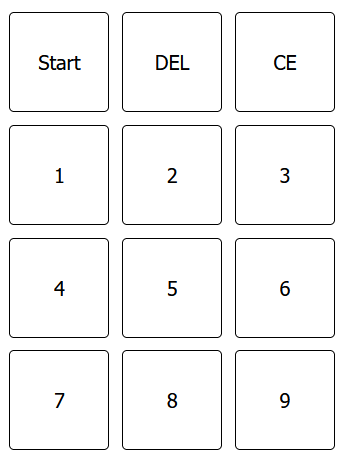
\includegraphics[width=0.2\textwidth]{images/NumPad.png}}%
	\qquad
	\subfloat[][]{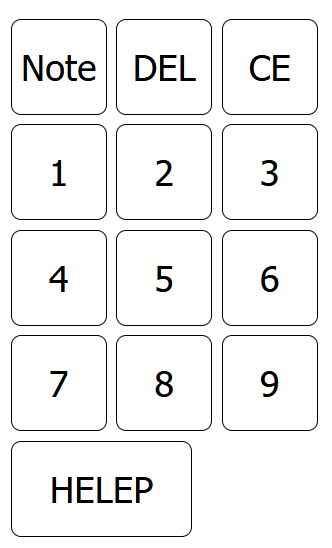
\includegraphics[width=0.2\textwidth]{images/NumPadHelp.png}}%
	\caption{Veränderung des NumPad nach Starten}%
\end{figure}

Mit den Ziffern des NumPad können, wie mit den Zahlen auf der Tastatur, Zahlen in das Sudoku eingetragen werden. Für die bessere Nutzung an einem Computer wird die Eingabe über das NumPad auf der Tastatur oder über die obere Zahlenreihe auf der Tastatur ermöglicht.

\subsection{Funktionalitäten Board}
Auch für das Board gibt es mehrere Funktionalitäten. Es gibt mehrere Möglichkeiten eine oder mehrere Zellen auszuwählen. Um die Zelle auf der man sich aktuell befindet ist eine bunte Umrandung. Diesen Curser kann man mit den Pfeiltasten bewegen. Wenn eine Zahl gedrückt wird, dann wird diese immer in der Zelle eingetragen auf der sich der Curser gerade befindet. Sobald die Zahl eingetragen wird springt der Cursor auf die nächste Zelle. Dem Nutzer ist es zudem möglich durch einen Mausklick mehrere Zellen auszuwählen. Die ausgewählten Zellen sind dann grau gefärbt. Wenn man die Markierung einer Zelle wieder rückgängig machen möchte, ist dies durch nochmaliges klicken möglich. 

In der Abbildung \ref{fig:Markierungen} sieht man das der Cursor ganz oben links auf der ersten Zelle (1, A) ist. Zudem sind mehrere Felder ausgewählt und daher grau hinterlegt.

\begin{figure}[htbp]
	\centering
	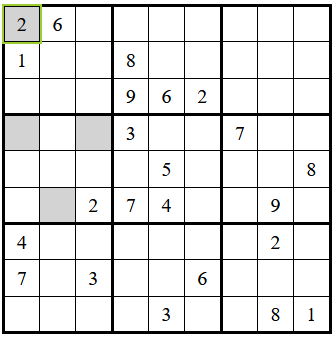
\includegraphics[width=0.3\textwidth]{images/Markierungen.png}
	\caption{Abbildung der möglichen Markierungsvarianten}
	\label{fig:Markierungen}
\end{figure}

Zahlen die vor dem Starten auf dem Sudokuboard eingetragen werden, werden mit dem Starten Blau markiert. Diese Zahlen können ab diesem Zeitpunkt nicht mehr überschrieben werden. Für den Fall, dass bei einem bereits gestartetem Sudoku eine inkorrekte Zahl eingetragen wird, so wird diese Rot markiert.


\section{Abstufungen der Hilfestellungen}
Die Anforderung an die verschiedenen Abstufungen der Hilfestellung wird hauptsächlich über das Frontend umgesetzt. Im Backend werden dafür nur die relevanten Informationen gesammelt. Im Folgenden wird die Abstufung und Umsetzung der Hilfestellungen erläutert und anhand von Beispielen gezeigt.

\subsection{Erste Hilfestellung}

Die erste Hilfestellung besteht daraus die anzuwendende Technik auf dem Frontend anzuzeigen und relevante Zellen zu markieren.  In dem Codebeispiel \ref{lst:help0} ist die Umsetzung dafür beschrieben.

\begin{lstlisting}[caption={Erste Hilfestellung}, label={lst:help0}]
	socket.on('help0', function (technique_result) {
		$("#technique-name").text(technique_result['name']);
		$("#technique-explanation").text("");
		colorCells(technique_result['primaryCells'], 'rgb(255,216,115)');
		colorCells(technique_result['secondaryCells'], 'rgb(181,216,244)');
	});
\end{lstlisting}

Es wird der Klasse \textit{technique-name} die Technik übergeben und über \textit{colorCells} können betroffene Zellen auf dem Board in verschiedenen Farben markiert werden. Diese Markierungen und das Anzeigen des Technik Namen ist in Abbildung \ref{fig:Help1} dargestellt. Die Zellen können in unterschiedlich eingefärbt werden, abhängig davon wie relevant sie für eine Technik sind. In den meisten Fällen haben die \textit{primaryCells} eine besondere Bedeutung für eine Technik und sind darauf ausgelegt zuerst aufzufallen. Die \textit{secondaryCells} haben aber auch eine Bedeutung für eine Technik weisen dabei aber eher auf den Grund hin, weshalb eine Technik angewendet werden kann oder in welchen Units die Technik gefunden wurde.

\begin{figure}[htbp]
	\centering
	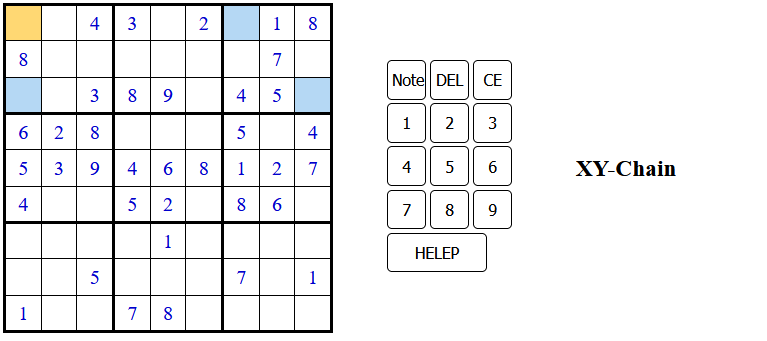
\includegraphics[width=0.8\textwidth]{images/Help1.png}
	\caption{Darstellung der ersten Hilfestellung}
	\label{fig:Help1}
\end{figure}

\subsection{Zweite Hilfestellung}
Mit der zweiten Hilfestellung werden relevante Kandidaten markiert. Im Falle der Kandidaten gibt es erneut zwei unterschiedliche Markierungen. Ein Teil dieser Hilfestellung ist das Anzeigen der Kandidaten, für den Fall dass dies nicht bereits der Fall ist. 

\begin{lstlisting}[caption={Zweite Hilfestellung}, label={lst:help1}]
	socket.on('help1', function (technique_result) {
		if (!candidatesVisible) {
			candidatesVisible = !candidatesVisible;
			$('#candidate').css('color', 'red');
		}
		colorCandidates(technique_result['crossOuts'], 'red');
		colorCandidates(technique_result['highlights'], 'lime');
	});

\end{lstlisting}

Kandidaten die für eine Lösungstechnik Relevanz haben können mittels der Funktion \textit{colorCandidates} markiert werden. Kandidaten die aufgrund der Technik heraus gestrichen werden können, werden auf dem Sudokuboard Rot markiert. Kandidaten auf denen eine Technik aufbaut werden grün hervorgehoben. Die Umsetzung wird in dem Codebeispiel \ref{lst:help1} beschrieben und das Ergebnis in der Abbildung \ref{fig:Help2} dargestellt.

\begin{figure}[htbp]
	\centering
	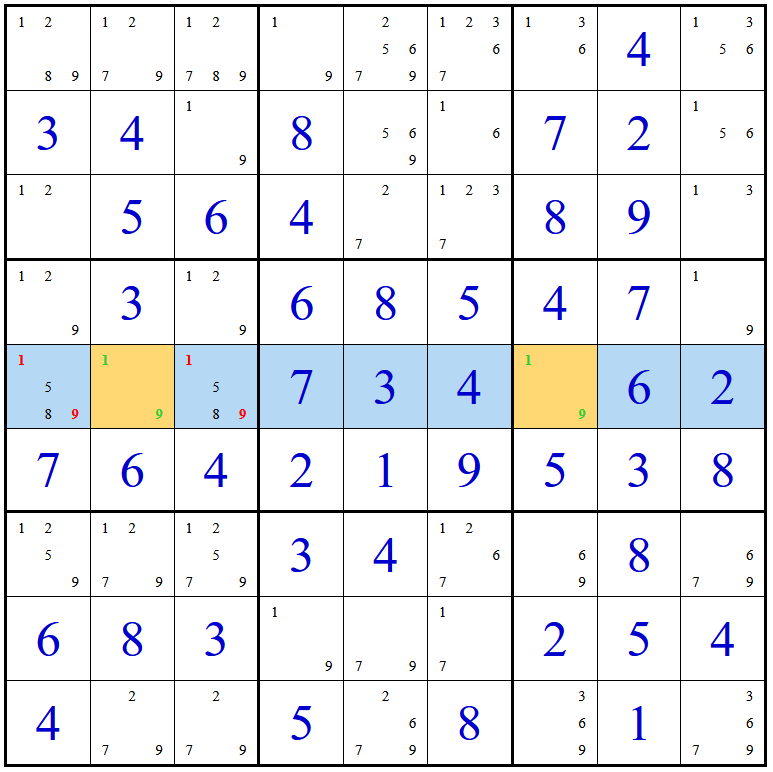
\includegraphics[width=0.5\textwidth]{images/Help2.png}
	\caption{Darstellung der zweiten Hilfestellung}
	\label{fig:Help2}
\end{figure}

\subsection{Dritte Hilfestellung}
Die dritte Hilfestellung besteht aus einer Erklärung der Technik anhand des aktuellen Sudokus. Die Erläuterung wird dabei unter dem Technikname in der Klasse \textit{technique-explanation} in einem <p> Element angezeigt. Diese Hilfestellung wurde analog zu dem Technikname in dem Codebeispiel \ref{lst:help0} umgesetzt.

\subsection{Vierte Hilfestellung}
Nachdem das Programm dem Nutzer über mehrere Schritte geholfen hat die Technik zu finden und gegebenenfalls nachzuvollziehen, wird mit der letzten Hilfestellungen die Technik ausgeführt. Rot eingefärbten Kandidaten vom Board entfernt. Außerdem werden alle Markierungen mit der Funktion \textit{resetCellColor()}, wie in dem Codebeispiel \ref{lst:help3} gezeigt, zurückgesetzt und der Techniktitel und die Beschreibung entfernt. 

\begin{lstlisting}[caption={Vierte Hilfestellung}, label={lst:help3}]
	socket.on('help3', function () {
		if (!candidatesVisible) {
			candidatesVisible = !candidatesVisible;
			$('#candidate').css('color', 'red');
		}
		$("#technique-name").text("");
		$("#technique-explanation").text("");
		resetCellColor();
	});

\end{lstlisting}

\section{Fertig gelöstes Sudoku}
Dem Nutzer wird sobald alle Zellen auf dem Board korrekt ausgefüllt wurden, über das Textfeld angezeigt, dass er das Sudoku korrekt gelöst hat.